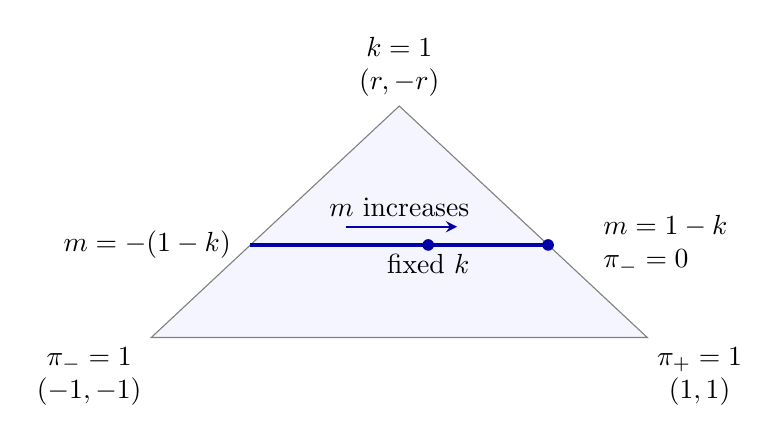
\begin{tikzpicture}[scale=1.05,>=stealth]
\coordinate (N) at (-3,0);
\coordinate (P) at (3,0);
\coordinate (C) at (0,2.8);
\fill[blue!4] (N)--(P)--(C)--cycle;
\draw[gray] (N)--(P)--(C)--cycle;
\node[below left,align=center] at (N) {$\pi_-=1$\\$(-1,-1)$};
\node[below right,align=center] at (P) {$\pi_+=1$\\$(1,1)$};
\node[above,align=center] at (C) {$k=1$\\$(r,-r)$};
\draw[very thick,blue!65!black] (-1.8,1.12)--(1.8,1.12);
\draw[->,thick,blue!65!black] (-.65,1.34)--(.7,1.34);
\node[above] at (0,1.34) {$m$ increases};
\fill[blue!65!black] (.35,1.12) circle (2pt);
\node[below] at (.35,1.12) {fixed $k$};
\fill[blue!65!black] (1.8,1.12) circle (2pt);
\node[right,align=left] at (2.35,1.12) {$m=1-k$\\$\pi_-=0$};
\node[left] at (-1.92,1.12) {$m=-(1-k)$};
\end{tikzpicture}
